\documentclass[11pt]{article}

\usepackage[T1]{fontenc}
\usepackage[utf8]{inputenc}
\usepackage{lmodern}
\usepackage[margin=1in]{geometry}
\usepackage{amsmath}
\usepackage{booktabs}
\usepackage{array}
\usepackage{enumitem}
\usepackage{microtype}
\usepackage{graphicx}
\usepackage{tikz}
\usetikzlibrary{arrows.meta, positioning, shapes.geometric, fit, calc}
\usepackage[natbibapa]{apacite}
\usepackage[hidelinks]{hyperref}

\setlength{\parskip}{0.4em}
\setlength{\parindent}{0pt}

% shared diagram styles (grayscale, matches the report's monochrome look)
\tikzset{
  fnode/.style={draw, rounded corners, align=center, font=\footnotesize,
    inner sep=4pt, minimum height=8mm, fill=black!3},
  dnode/.style={draw, align=center, font=\footnotesize,
    inner sep=4pt, minimum height=8mm, fill=black!10},
  dec/.style={draw, diamond, aspect=2.2, align=center, font=\scriptsize,
    inner sep=0pt, fill=black!5},
  term/.style={draw, rounded corners=6pt, align=center, font=\footnotesize\bfseries,
    inner sep=4pt, minimum height=8mm, fill=black!14},
  arr/.style={-{Stealth[length=2mm]}, semithick},
  darr/.style={-{Stealth[length=2mm]}, semithick, dashed},
  elbl/.style={font=\scriptsize\itshape, fill=white, inner sep=1pt},
}

\title{\textbf{pgrep}: A Physics GRE Preparation System with Separated, Calibrated Readiness Scores}
\author{Frank Gonzalez}
\date{July 2026}

\begin{document}
\maketitle

\begin{abstract}
pgrep is a desktop and mobile study system for the Physics GRE (PGRE). The PGRE
rewards problem solving over fact recall, so a recall-only flashcard tool is the
wrong instrument for it. pgrep addresses this with four pieces of work. First, an
in-engine study selector reorders due items by exam value, blueprint weight times
topic weakness, without altering any scheduling state. Second, three separated and
calibrated scores report what a learner can recall now (Memory), whether they can
apply it to a new question (Performance), and what they would likely score
(Readiness), each with an explicit range and an abstain rule. Third, an AI item
layer generates cards, misconception-first multiple-choice problems, and a
scaffold-fade tutor, each citing a named open source or refusing, and each gated by
a pre-registered gold-set test and a leakage firewall. Fourth, every model is
evaluated on held-out data against a bar set in advance, and the negatives are
reported. On held-out review logs, Memory calibrates to a Brier score of 0.234 and
beats a base-rate baseline. A simulated ablation shows the selector beats massed
practice in every configuration and beats stock scheduling at realistic study
budgets. The AI layer beats keyword, vector, and naive-distractor baselines with
confidence intervals excluding zero, although two absolute quality cutoffs remain
just short. pgrep runs and scores with AI switched off.

\textbf{Keywords:} spaced repetition, exam readiness, calibration, interleaving,
educational data mining, retrieval-augmented generation, item generation.
\end{abstract}

\section{Introduction}

Preparing for a single high-stakes exam is a measurement problem as much as a study
problem. A learner needs to know not only whether a fact is in memory, but whether
they can deploy it on a novel question under time pressure, and what score that
predicts. The Physics GRE is a sharp instance. It is one hundred five-choice
multiple-choice questions in 170 minutes, scored 200 to 990 with a one-quarter-point
penalty for wrong answers, and its content
blueprint has been stable for two decades: Mechanics 20\%, Electromagnetism 18\%,
Quantum 13\%, and six smaller areas. The exam is problem-solving-heavy and
fact-recall-light. That single fact reframes the tooling. The intended user is a
post-undergraduate physics student who has already met the material and wants to raise a
score, not a novice meeting it for the first time, which tilts the design toward
practice and measurement and away from teaching. Flashcards, the default
study technology, train recall, and recall is the weakest predictor of the skill the
PGRE actually tests.

The gap between the two is not incidental. \citet{soderstrom2015} distinguish
\emph{learning}, a durable and transferable change, from \emph{performance}, what a
learner can do right now, and show that the two often move in opposite directions.
A study method can inflate in-session performance while doing little for durable
transfer. A study tool that measures only recall therefore reports a number that
feels like readiness but is not. pgrep is built on the premise that three different
questions need three different instruments. Can you recall a fact now (Memory)? Can
you apply it to a question you have not seen (Performance)? What would you score
(Readiness)? These are kept as three separate numbers, never collapsed, because
recall does not imply transfer. A learner can have strong Memory on a topic and weak
Performance on it, having memorized a result without being able to choose it on a fresh
problem, and folding the two into one number would hide exactly the gap the exam probes.

The second premise is that honesty is a design property, not a disclaimer. Every
number pgrep shows carries a likely range, a coverage figure, and an abstain rule
that refuses to render a score when the data behind it is too thin. A readiness
estimate over a topic the learner has never practiced is not a low number, it is no
number, and the surface says which topics are missing. This posture, that abstaining
beats bluffing, runs through the whole system and through this report.

pgrep is a working desktop application with a native mobile companion, sharing one
study engine with two-way sync. It reuses a proven memory model for scheduling and
builds the exam-readiness layer on top. This report describes the system and
evaluates it. The contributions are four.

\begin{enumerate}[leftmargin=1.4em]
\item \textbf{An in-engine exam-value selector.} A new review-card ordering, computed
inside the study engine, reorders due items by blueprint weight times topic weakness,
within a desirable-difficulty band, without mutating any scheduling state.
\item \textbf{Three separated, calibrated scores.} Memory, Performance, and Readiness,
each with an 80\% central interval and an abstain rule, and each validated against
held-out outcomes rather than asserted.
\item \textbf{A provenance-gated AI item layer.} Card generation, misconception-first
problem generation, and a scaffold-fade tutor, each of which cites a named open-corpus
source or refuses, and each gated by a pre-registered gold-set test and a leakage
firewall.
\item \textbf{A reproducible held-out evaluation.} Every model is measured on held-out
data against a bar fixed before results were seen, and the negatives are reported
alongside the wins.
\end{enumerate}

The remainder of the report covers the foundation pgrep reuses, the system at a
glance, the study selector, the three-score model, the AI layer, the evaluation, and
a discussion of what the evidence does and does not support.

\section{Background and Foundation}

\subsection{The reused engine}

pgrep is built by reusing the engine of an open-source spaced-repetition application
(Anki) and replacing its interface and its study logic. The reuse is deliberate and
bounded. What pgrep inherits is the memory model, the collection store and its review
log, the two-way sync system, and the local web-host mechanism that serves the user
interface. What pgrep adds, and what this report is about, is everything above that
line: the exam-value selector, the three-score model, the AI item layer, the
evaluation harness, the desktop surfaces, and the mobile companion. The reused engine
is licensed under the AGPL, and pgrep preserves that license and its attribution.

The memory model is worth naming because the Memory score depends on it. The engine
ships FSRS, a modern three-component model of memory (difficulty, stability,
retrievability) whose forgetting curve gives, for any card at any moment, a predicted
probability of recall. On a large public benchmark of review histories, FSRS is the
strongest non-neural scheduler, ahead of the older SM-2 heuristic and of half-life
regression \citep{settles2016}, and it descends from a line of work that frames
spaced repetition as an optimization problem \citep{tabibian2019, yesucao2022,
fsrs2024}. pgrep does not modify the memory model. It consumes the model's
retrievability estimate and builds selection and scoring on top of it.

\subsection{The learning-science basis}

Four findings from the learning-science literature shape pgrep's features. Each is a
mechanism pgrep implements, not a result pgrep claims for itself.

\textbf{Interleaving.} Practicing related topics in a mixed order, rather than in
blocks, improves later performance on novel problems, often substantially. With
spacing held fixed, interleaved mathematics practice roughly doubled next-day test
scores \citep{taylor2010}, and the benefit extends to problems that are not
superficially similar, with large effects reported, a Cohen's $d$ near $1.0$ in one
multi-week study \citep{rohrer2007, rohrer2014}. In undergraduate physics, mixed
homework raised surprise novel-problem scores by 50 to 125 percent \citep{samani2021},
and meta-analyses report medium effects that are largest when the concepts are
confusable \citep{firth2021, sana2022}. The mechanism matters
here: interleaving forces the learner to choose a strategy from the problem itself,
training the discrimination the PGRE demands. Learners reliably misjudge its value,
preferring blocked study that feels easier \citep{kornell2008}.

\textbf{The generation effect.} Material a learner produces is remembered better than
material they read, even when the content is identical, with a meta-analytic effect
around $d = 0.40$ \citep{slamecka1978, bertsch2007}. User-generated flashcards
outperform premade ones on both memory and application \citep{pan2022flashcards}.
pgrep uses this to gate AI card generation behind an authoring step, so the learner
pays the generative cost at novel-concept formation before the system amortizes that
style across the rest of the deck.

\textbf{Productive struggle with consolidation.} Attempting a problem before receiving
help, then consolidating with feedback, aids transfer \citep{kapur2008, kapur2016},
subject to the caveat that heavy guidance backfires as prior knowledge grows
\citep{kalyuga2007}. In a randomized trial with about one thousand students,
unguarded access to a general assistant reduced learning, whereas a guardrailed tutor
did not \citep{bastani2024}. Help must therefore be scaffolded, must make the learner
produce the reasoning \citep{chi1989}, and must not leak the answer, since a large
share of naive AI hints simply solve the task for the student. Retrieving principles
before solving primes the solving itself, with an effect near $d = 0.4$
\citep{roediger2006, gjerde2022}, and completion and worked-example structure manage
cognitive load \citep{sweller1988, renkl2003}.

\textbf{Calibration over confidence.} The honest move is to make the system's own
predictions calibrated and visible, not to harvest the learner's subjective
confidence. This is measured with proper scores and reliability diagrams
\citep{brier1950, degroot1983, guo2017}.

\section{System Overview}

pgrep is organized around three co-equal pillars that map onto the three scores, and
a single study loop that feeds them (Figure~\ref{fig:system}).

\begin{figure}[t]
\centering
\resizebox{\textwidth}{!}{%
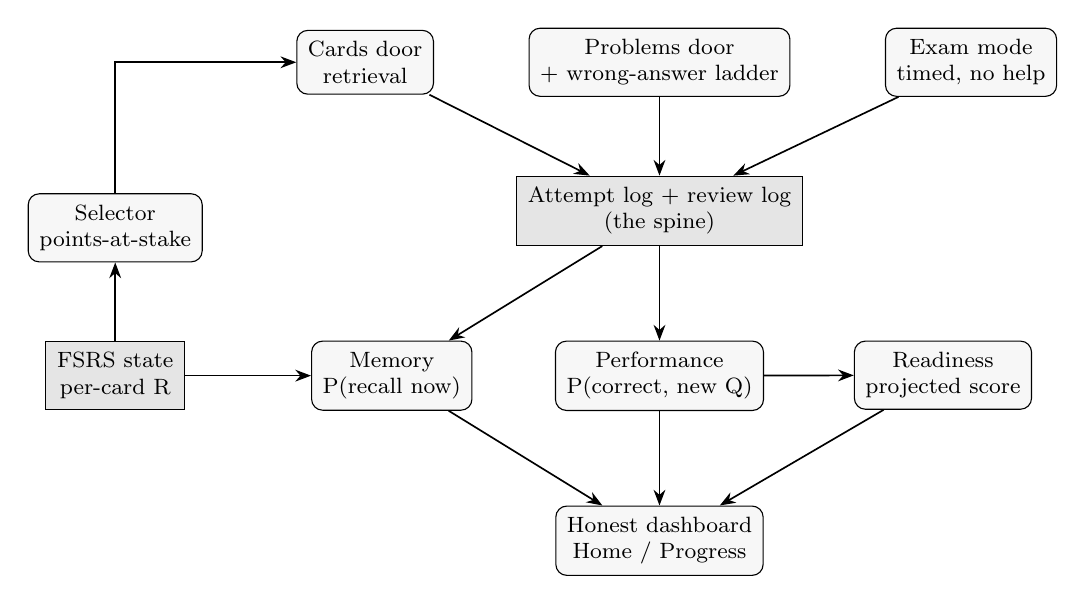
\begin{tikzpicture}[node distance=8mm and 12mm]
\node[fnode] (cards) {Cards door\\retrieval};
\node[fnode, right=of cards] (probs) {Problems door\\+ wrong-answer ladder};
\node[fnode, right=of probs] (exam) {Exam mode\\timed, no help};
\node[dnode, below=10mm of probs] (log) {Attempt log + review log\\(the spine)};
\draw[arr] (cards) -- (log);
\draw[arr] (probs) -- (log);
\draw[arr] (exam) -- (log);
\node[fnode, below=12mm of log, xshift=-34mm] (mem) {Memory\\P(recall now)};
\node[fnode, below=12mm of log] (perf) {Performance\\P(correct, new Q)};
\node[fnode, below=12mm of log, xshift=36mm] (ready) {Readiness\\projected score};
\draw[arr] (log) -- (mem);
\draw[arr] (log) -- (perf);
\draw[arr] (perf) -- (ready);
\node[dnode, left=16mm of mem] (fsrs) {FSRS state\\per-card R};
\node[fnode, above=10mm of fsrs] (sel) {Selector\\points-at-stake};
\draw[arr] (fsrs) -- (mem);
\draw[arr] (fsrs) -- (sel);
\draw[arr] (sel) |- (cards);
\node[fnode, below=12mm of perf] (dash) {Honest dashboard\\Home / Progress};
\draw[arr] (mem) -- (dash);
\draw[arr] (perf) -- (dash);
\draw[arr] (ready) -- (dash);
\end{tikzpicture}%
}
\caption{System data flow. The attempt log and review log are the spine: every card
review, problem attempt, and exam item feeds them, they drive the three scores and the
honest dashboard, and the FSRS state feeds both the Memory score and the
points-at-stake selector that orders the study doors.}
\label{fig:system}
\end{figure}

\textbf{The three pillars.} Cards build Memory through retrieval. Problems build
Performance through application, with reasoning-first help. Timed mocks build
Readiness under exam conditions. The pillars are kept co-equal on purpose. The thesis
that the PGRE rewards problem solving is not enforced by a hand-tuned weighting, it
falls out of the engine and the study mix, so no pillar is special-cased.

\textbf{The study loop.} A session runs as two doors, never one shuffled queue,
because mixing cards and problems within a single queue has no support in the
literature. Inside each door, topics are interleaved. On the Problems door, the
learner commits an answer before any help is offered, which preserves the
attempt-before-help structure that productive struggle requires. A short adaptive
diagnostic places each topic as strong or rusty at first run, and a coverage-aware
daily mix suggests the next best thing to study. A Focus drill reuses both doors scoped
to a single topic for targeted repair, and every Problems session ends with a short
synthesis of the patterns across its problems, the consolidation step that productive
struggle requires. Exam mode is kept separate as the measuring instrument, timed and
help-free, so the number used to estimate readiness is never inflated by the help that
makes everyday practice productive.

\textbf{Surfaces and platforms.} The desktop application presents six custom
surfaces: Home (the three scores at a glance), Study (the two doors plus a timed exam
mode), Progress (coverage and model calibration), Diagnostic, Library (authoring and
generation), and Settings. A native mobile companion mirrors Home and Study on the
same shared engine, and the two devices sync two-way. The desktop and mobile hosts
are thin shells over one engine and one remote-procedure surface, so parity is
structural rather than duplicated.

\textbf{The attempt log is the spine.} Every graded event, a card review, a problem
attempt, an exam item, is recorded. Card reviews ride the engine's existing review
log. Problem attempts, which carry richer data (the selected option, the depth
reached in the help ladder, sub-goal productions, timing, and a session id), are
stored as an append-only log of immutable notes. This choice, storing the log as
notes rather than as a custom database table, lets it ride the engine's existing
sync for free and merge cleanly across devices, at the cost of a little analytic
overhead. The log is the single source that feeds the selector, the three scores, and
the calibration dashboard.

\subsection{Architecture and data model}

Desktop and mobile are two thin hosts over one engine. On the desktop, a local web
server serves the interface, a native window displays it, and the page calls the
engine through the same remote procedures the mobile app uses. The mobile companion is
a native application that drives the shared engine through a small
foreign-function-interface layer. Because both hosts call one engine and one procedure
surface, including the exam-value selector, parity between devices is structural rather
than duplicated, and a study session behaves the same on either.

The attempt log's storage was a deliberate decision with a documented evolution path,
recorded as \emph{A now, C-ready}. Storing each attempt as an immutable note (option
A) lets the log ride the engine's note sync for free and merge across devices by
identifier, at the cost of parsing string fields for analytics. A custom database
table (option B) would give faster typed queries but would require writing custom sync
inside the engine, the project's most heavily weighted requirement, so it was rejected.
A local recomputable cache folded from the notes (option C) recovers that speed with no
sync risk, and is pre-engineered but deferred until the fold measurably slows. Five
invariants make the later flip to C free: notes are immutable and self-contained, event
identity is the note's own identifier, the payload is one JSON blob plus a few hot
fields, all analytics pass through a single read seam, and the cache is a pure fold that
never touches sync.

\section{The Study Selector}

The first pillar's engine change is a new way to order the cards that are due on a
given day. The design goal is simple to state: when there are more due cards than the
daily limit allows, spend the limit on the cards that matter most for the exam, and
present them in an interleaved order.

\subsection{Why this is a real engine change}

A naive implementation would gather the day's due cards in some default order and
re-sort them in the interface. That does not work here, because the engine applies
the daily review limit \emph{during} the database query that gathers cards, ordered
by a fixed clause. The cards that matter most might never be gathered before the
limit cuts the list off. Ordering by exam value therefore requires a change inside
the engine, not a cosmetic sort after the fact.

pgrep adds a new review-card ordering, \texttt{ReviewCardOrder::PointsAtStake}, and a
second pass in the engine that gathers all due reviews, scores them, and then
truncates to the limit. This gather-then-limit structure is the substantive change
(Figure~\ref{fig:selector}).

\begin{figure}[t]
\centering
\resizebox{\textwidth}{!}{%
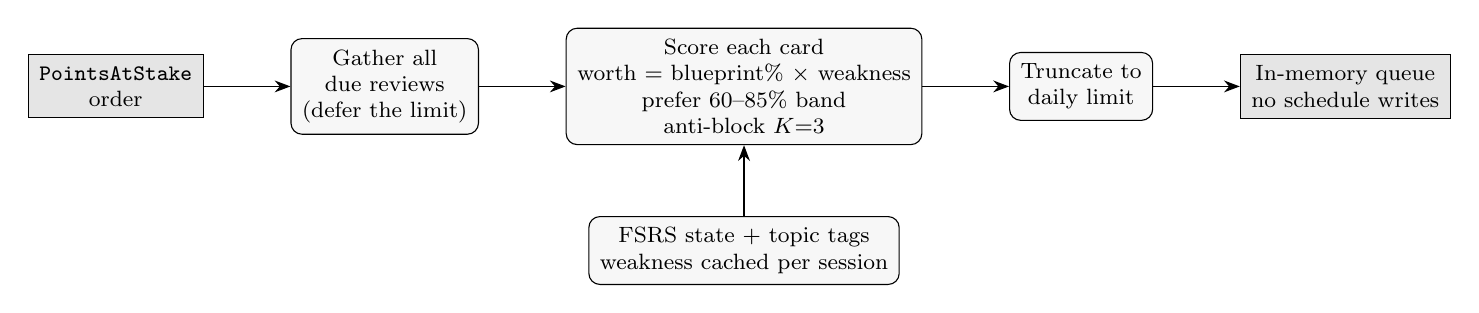
\begin{tikzpicture}[node distance=7mm and 11mm]
\node[dnode] (po) {\texttt{PointsAtStake}\\order};
\node[fnode, right=of po] (gather) {Gather all\\due reviews\\(defer the limit)};
\node[fnode, right=of gather] (score) {Score each card\\worth $=$ blueprint\% $\times$ weakness\\prefer 60--85\% band\\anti-block $K{=}3$};
\node[fnode, right=of score] (trunc) {Truncate to\\daily limit};
\node[dnode, right=of trunc] (q) {In-memory queue\\no schedule writes};
\draw[arr] (po)--(gather); \draw[arr] (gather)--(score); \draw[arr] (score)--(trunc); \draw[arr] (trunc)--(q);
\node[fnode, below=9mm of score] (in) {FSRS state $+$ topic tags\\weakness cached per session};
\draw[arr] (in)--(score);
\end{tikzpicture}%
}
\caption{The points-at-stake selector as a gather-then-limit second pass. It gathers
every due review, scores each by exam value within a difficulty band and with
anti-blocking, and truncates to the daily limit, all in memory, so no scheduling state
is written.}
\label{fig:selector}
\end{figure}

\subsection{The score}

Each due card is scored by the exam value at stake in reviewing it:
\[
\text{worth}(\text{card}) = \text{blueprint}\%\big(\text{topic}\big) \times \text{weakness}\big(\text{topic}\big),
\qquad
\text{weakness}(\text{topic}) = 1 - \bar{R}_{\text{topic}},
\]
where $\bar{R}_{\text{topic}}$ is the mean predicted retrievability over that topic's
due cards, and blueprint\% is the official PGRE weight for the topic's area. Weakness
is computed from the memory model alone, so the selector needs no attempt-log
dependency and the per-topic weakness map can be cached once per session. Among the
scored cards, the selector prefers those in a desirable-difficulty band of roughly 60
to 85\% predicted success \citep{wilson2019, metcalfe2005}, and it applies an
anti-blocking rule that allows at most three consecutive cards from the same area, so
the emitted order stays interleaved.

Computing weakness from the memory model has a practical payoff. The per-topic weakness
map is built once per session and cached, so the second pass stays well under the
interface's responsiveness budget even on a large collection. The shipped weighting is
fixed, which is the graded minimum. A planned extension anneals the balance between
worth and the difficulty band along a dial driven by time to test and coverage,
shifting from a learning emphasis when the exam is far toward a triage emphasis as it
nears. That loop steers study only, never the held-out measurement, so it can never
grade its own homework.

\subsection{The safe seam}

The selector reorders the in-memory set of due cards and nothing more. It never
mutates the scheduling fields (\texttt{due}, \texttt{interval}, or
\texttt{memory\_state}), never writes collection data, and never creates an undo
entry. Queues live in memory and are rebuilt each session, so reordering them writes
nothing and cannot corrupt the collection. This is what lets a genuine engine change
sit safely inside a scheduler the authors did not write: scheduling, undo, and sync
are untouched, and the memory model's validity is preserved by construction. The
change is covered by three engine-level tests and one integration test.

\section{The Three-Score Model}

The core of pgrep is three separate numbers, each answering a different question,
each reported with a range and an abstain rule. The design principle is that
uncertainty is first-class and standardized: every range is an 80\% central interval,
computed the same way everywhere, and every score refuses to render when its data is
too thin. Three further principles hold across all three. Each number carries its own
honesty, a point estimate, a likely range, a data-sufficiency read, and a last-updated
time, so no bare number appears without its evidence. All three are pure arithmetic over
the memory model and the attempt log, with no model in the loop, so both apps produce
all three scores with AI switched off. And each reuses the engine's own primitives where
it can, so Memory and the selector's weakness term, for one, are the same quantity and
cannot disagree. Table~\ref{tab:scores} summarizes the three.

\begin{table}[t]
\centering
\small
\begin{tabular}{@{}p{2.0cm}p{3.3cm}p{3.6cm}p{4.2cm}@{}}
\toprule
\textbf{Score} & \textbf{Predicts} & \textbf{Model} & \textbf{Abstains when} \\
\midrule
Memory & Recall now & Blueprint-weighted FSRS retrievability & A topic has fewer than 5 reviewed cards \\
Performance & Correct on a new question & PFA calibrated logistic over 4 features & A topic has fewer than about 8 clean attempts \\
Readiness & Projected scaled score & Expected raw mapped to the 200--990 scale & Coverage is under 70\% of blueprint weight \\
\bottomrule
\end{tabular}
\caption{The three scores. Each is a distinct construct, model, and abstain rule.}
\label{tab:scores}
\end{table}

\begin{figure}[t]
\centering
\resizebox{\textwidth}{!}{%
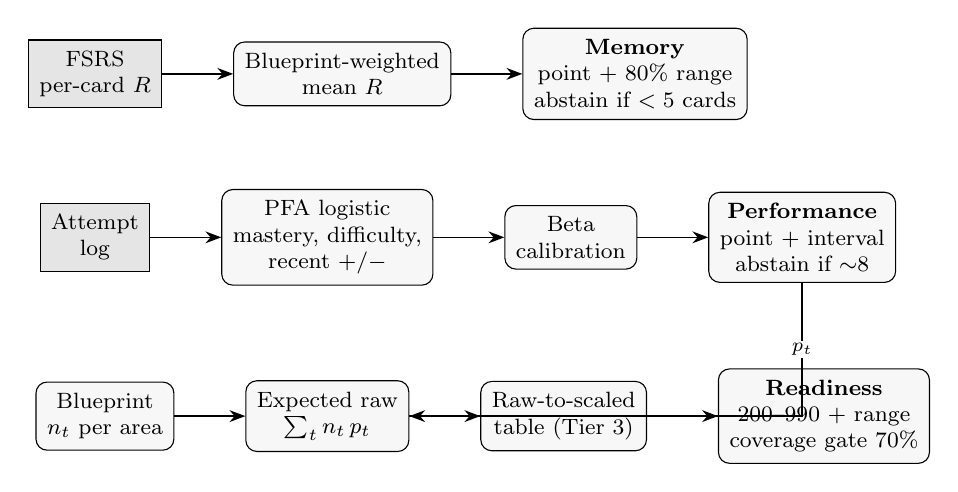
\begin{tikzpicture}[node distance=6mm and 9mm]
\node[dnode] (fr) {FSRS\\per-card $R$};
\node[fnode, right=of fr] (mw) {Blueprint-weighted\\mean $R$};
\node[fnode, right=of mw] (mem) {\textbf{Memory}\\point $+$ 80\% range\\abstain if $<5$ cards};
\draw[arr] (fr)--(mw); \draw[arr] (mw)--(mem);
\node[dnode, below=12mm of fr] (al) {Attempt\\log};
\node[fnode, right=of al] (pfa) {PFA logistic\\mastery, difficulty,\\recent $+/-$};
\node[fnode, right=of pfa] (beta) {Beta\\calibration};
\node[fnode, right=of beta] (perf) {\textbf{Performance}\\point $+$ interval\\abstain if ${\sim}8$};
\draw[arr] (al)--(pfa); \draw[arr] (pfa)--(beta); \draw[arr] (beta)--(perf);
\node[fnode, below=12mm of pfa] (raw) {Expected raw\\$\sum_t n_t\, p_t$};
\node[fnode, left=of raw] (bp) {Blueprint\\$n_t$ per area};
\node[fnode, right=of raw] (tab) {Raw-to-scaled\\table (Tier 3)};
\node[fnode, right=of tab] (ready) {\textbf{Readiness}\\200--990 $+$ range\\coverage gate 70\%};
\draw[arr] (bp)--(raw); \draw[arr] (raw)--(tab); \draw[arr] (tab)--(ready);
\draw[arr] (perf) |- (raw) node[elbl, pos=0.25]{$p_t$};
\end{tikzpicture}%
}
\caption{How the three scores are derived. Memory is a blueprint-weighted average of
FSRS retrievability; Performance is a calibrated logistic over attempt-log features;
Readiness maps the expected raw score, built from per-topic $p_t$ and blueprint question
counts $n_t$, through the official conversion table. Each carries an 80\% range and an
abstain rule.}
\label{fig:scores}
\end{figure}

\subsection{Memory}

Memory is the expected fraction of a learner's due and known cards they would recall
right now, weighted by the blueprint. It reuses the memory model directly: each
card's predicted retrievability is read from the engine, averaged per topic, and
combined across topics by blueprint weight. Because the number of cards recalled is a
sum of independent, non-identical Bernoulli trials, its distribution is
Poisson-binomial \citep{lecam1960}, which gives an analytic mean and variance and
hence the 80\% range. A topic with fewer than five reviewed cards shows ``not enough
cards yet'' rather than a number. By construction, Memory and the selector's weakness
term use the same primitive, so the score and the study order never disagree.

\subsection{Performance}

Performance is the probability of answering a new, unseen exam-style question
correctly, per topic and overall. This is transfer, not recall, so it is computed
from the attempt log rather than from the memory model. The model is Performance
Factors Analysis, a calibrated logistic regression that is the standard
education-data-mining approach to predicting next-item correctness
\citep{pavlik2009, cen2006}. It is preferred over Bayesian Knowledge Tracing,
which has known identifiability difficulties \citep{corbett1994}, and over deep
knowledge tracing, which is data-hungry and opaque at this scale \citep{piech2015}.
For a problem $j$ in topic $t$,
\[
P(\text{correct}) = \sigma\!\left(\beta_0 + \beta_m\, m_t - \beta_d\, d_j
+ \gamma_s\, s_t + \gamma_f\, f_t\right),
\]
where $m_t$ is topic mastery (mean retrievability), $d_j$ is the authored item
difficulty, and $s_t$ and $f_t$ are recency-weighted counts of recent successes and
failures, kept separate because successes and failures carry different weight
\citep{galyardt2014}. Response latency is used only to filter rapid-guess attempts
and to measure pace in the timed exam mode, not as a predictor, because in untimed
practice a slow answer is ambiguous. Coverage is used to widen the interval and to
gate Readiness, not as a predictor.

Two modeling choices are worth defending. First, the baseline the model must beat is
the per-topic base rate, the batting average, which is honest and robust and is what
the system falls back to with too little data. PFA earns its place only if it beats
that baseline \citep{gong2011}. Second, a full item-response or Rasch model was
rejected. With a single learner, item difficulty and learner ability are jointly
unidentifiable, and such models need roughly one to two hundred examinees per item
\citep{lord1980, embretson2000}. The authored difficulty tag gives most of the
difficulty-awareness without the estimation. Raw logistic scores are not
automatically calibrated, so a post-hoc beta calibration is fit on a held-out split
\citep{kull2017, platt1999}, chosen over alternatives that overfit at small sample
sizes. The 80\% interval comes from Bayesian partial pooling across topics
\citep{gelman2013}, and a topic abstains until its interval is tight enough, with about eight to ten clean
attempts as a starting proxy \citep{brown2001, peduzzi1996}.

\subsection{Readiness}

Readiness is the projected scaled score, in the PGRE's 200 to 990 band, with an
explicit range and a coverage figure. It leans on Performance, not Memory, because
the exam measures transfer. For each area, the per-topic probability $p_t$ from the
Performance model is combined with $n_t$, the number of exam questions that area
contributes under the blueprint. The expected raw score is $\sum_t n_t p_t$, again a
Poisson-binomial sum with an analytic mean and variance. The raw point and the raw
interval endpoints are then mapped through the official raw-to-scaled conversion table
from a real practice form, used as numeric constants only. The result is a scaled
point estimate and an 80\% scaled interval. Thin coverage widens the interval before it
trips the gate, so the range tightens as more of the exam is practiced, which is the
honest visual of readiness accruing.

Readiness is where honesty-by-construction is most visible. Coverage is the fraction
of blueprint weight whose topics have cleared the Performance data floor. If coverage
is under 70\%, Readiness abstains, states that not enough of the exam is covered yet,
and names the uncovered areas. A learner cannot manufacture a readiness number over a
part of the exam they have not practiced.

\section{The AI Layer}

The AI layer enriches the item pool. It is an upgrade, never a dependency: every path
has a working AI-off fallback, and an AI-off session loads none of the AI code. The
layer has one hard rule, that every generated output cites a named source from an
open corpus or is refused, and it is gated before anything ships.

\subsection{What it generates}

\textbf{Cards.} Card generation is pay-to-play, reflecting the generation effect. The
learner authors a conceptual seed first. If the bundled deck already covers that
subtopic, the AI stylizes the verified card into the learner's voice, with the facts
locked one-to-one. If the deck lacks the technique, the seed triggers gap-fill
generation of new cards, grounded in the corpus and gold-set gated. Import adds
breadth but never substitutes for authoring, because importing someone else's cards
yields no generation effect. Figure~\ref{fig:cardgen} shows the routing.

\begin{figure}[t]
\centering
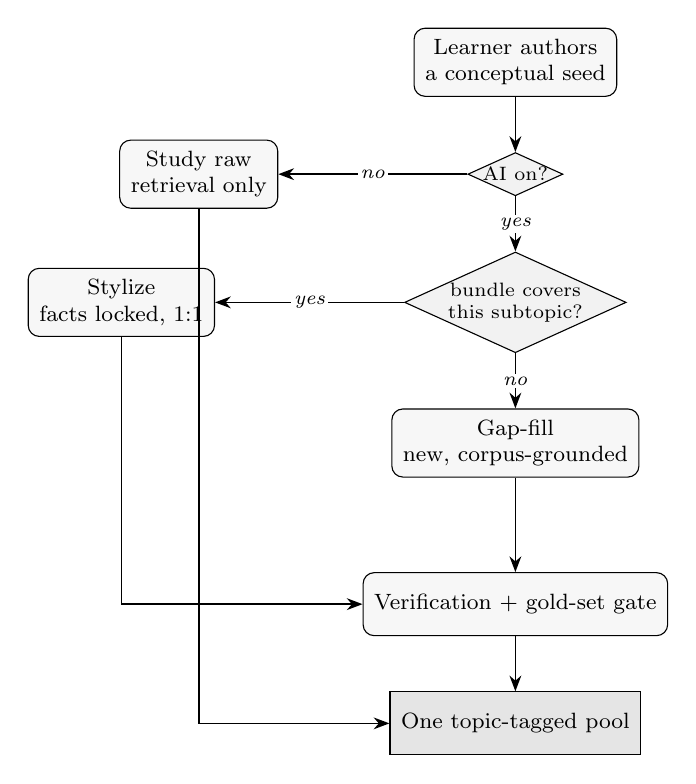
\begin{tikzpicture}[node distance=7mm and 10mm]
\node[fnode] (seed) {Learner authors\\a conceptual seed};
\node[dec, below=of seed] (aion) {AI on?};
\node[fnode, left=24mm of aion] (off) {Study raw\\retrieval only};
\node[dec, below=of aion] (cover) {bundle covers\\this subtopic?};
\node[fnode, left=24mm of cover] (styl) {Stylize\\facts locked, 1:1};
\node[fnode, below=of cover] (gap) {Gap-fill\\new, corpus-grounded};
\node[fnode, below=12mm of gap] (gate) {Verification $+$ gold-set gate};
\node[dnode, below=of gate] (pool) {One topic-tagged pool};
\draw[arr] (seed)--(aion);
\draw[arr] (aion) -- node[elbl]{no} (off);
\draw[arr] (aion) -- node[elbl]{yes} (cover);
\draw[arr] (cover) -- node[elbl]{yes} (styl);
\draw[arr] (cover) -- node[elbl]{no} (gap);
\draw[arr] (styl) |- (gate);
\draw[arr] (gap) -- (gate);
\draw[arr] (gate) -- (pool);
\draw[arr] (off) |- (pool);
\end{tikzpicture}
\caption{Card generation is pay-to-play. The learner authors a seed first; with AI on,
the system stylizes existing bundle cards where the deck already covers the subtopic and
gap-fills new, corpus-grounded cards where it does not. Everything passes verification
and the gold-set gate before entering the one shared pool.}
\label{fig:cardgen}
\end{figure}

\textbf{Problems.} The value and the risk of a multiple-choice problem sit in its
distractors. Naive generation asks the model for wrong answers and gets implausible
ones. pgrep uses misconception-first generation: name the specific error a student is
likely to make (a sign error, a wrong law, a unit slip, a limiting-case confusion),
then derive the distractor that error actually produces, and store the misconception
tag and rationale with each choice. Every generated problem also carries a solution
decomposition, ordered sub-goals with a rubric each, verified once at creation. A
problem without a verified decomposition does not ship. The misconception tags come from
a small taxonomy of recurring physics errors, and the stored rationale for each
distractor is what the tutor later teaches from, so the same annotation that makes a
problem hard also makes its help specific (Figure~\ref{fig:probgen}).

\begin{figure}[t]
\centering
\resizebox{0.95\textwidth}{!}{%
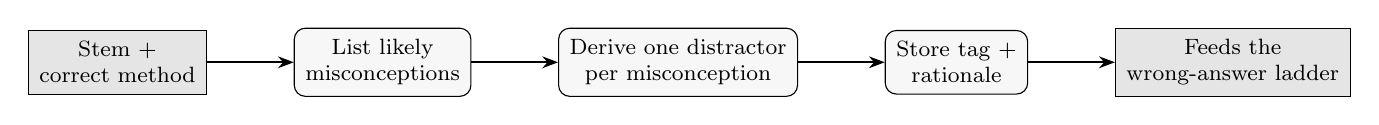
\begin{tikzpicture}[node distance=6mm and 11mm]
\node[dnode] (q) {Stem $+$\\correct method};
\node[fnode, right=of q] (mis) {List likely\\misconceptions};
\node[fnode, right=of mis] (der) {Derive one distractor\\per misconception};
\node[fnode, right=of der] (store) {Store tag $+$\\rationale};
\node[dnode, right=of store] (tut) {Feeds the\\wrong-answer ladder};
\draw[arr] (q)--(mis); \draw[arr] (mis)--(der); \draw[arr] (der)--(store); \draw[arr] (store)--(tut);
\end{tikzpicture}%
}
\caption{Misconception-first problem generation. Rather than asking for wrong answers,
the pipeline names the likely error, derives the distractor that error produces, and
stores the tag and rationale, which the tutor then teaches from.}
\label{fig:probgen}
\end{figure}

\textbf{The tutor.} When a learner misses a problem, a scaffold-fade ladder helps
without leaking the answer: a nudge, then sub-goal decomposition with self-explanation
over the stored decomposition, then a sibling worked example, then a full reveal with
explain-back. The ladder walks the stored, pre-verified sub-goals rather than
generating steps live, which makes it fast, reliable, and AI-off capable. A giveaway
verifier checks every AI hint and refuses rather than reveal the answer, addressing
the leakage that unguarded assistance introduces \citep{bastani2024}. With AI off, the
same ladder runs as reveal-and-self-compare. Figure~\ref{fig:ladder} shows the ladder.

\begin{figure}[t]
\centering
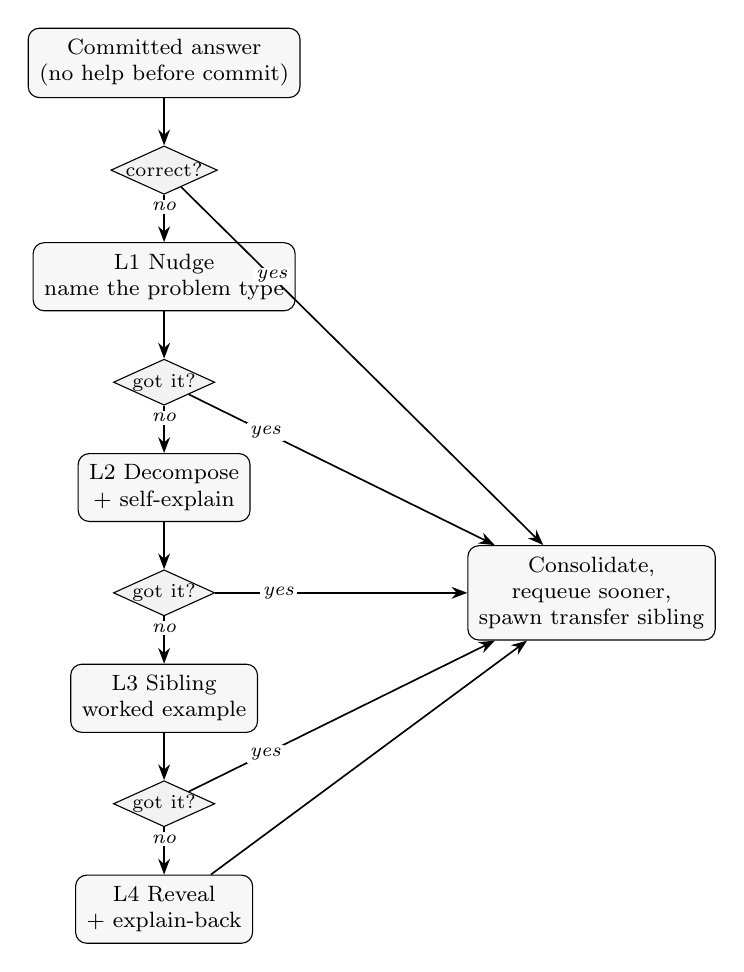
\begin{tikzpicture}[node distance=6mm and 26mm]
\node[fnode] (commit) {Committed answer\\(no help before commit)};
\node[dec, below=of commit] (correct) {correct?};
\node[fnode, below=of correct] (l1) {L1 Nudge\\name the problem type};
\node[dec, below=of l1] (g1) {got it?};
\node[fnode, below=of g1] (l2) {L2 Decompose\\$+$ self-explain};
\node[dec, below=of l2] (g2) {got it?};
\node[fnode, below=of g2] (l3) {L3 Sibling\\worked example};
\node[dec, below=of l3] (g3) {got it?};
\node[fnode, below=of g3] (l4) {L4 Reveal\\$+$ explain-back};
\node[fnode, right=32mm of g2] (cons) {Consolidate,\\requeue sooner,\\spawn transfer sibling};
\draw[arr] (commit)--(correct);
\draw[arr] (correct) -- node[elbl,near start]{no} (l1);
\draw[arr] (l1)--(g1);
\draw[arr] (g1) -- node[elbl,near start]{no} (l2);
\draw[arr] (l2)--(g2);
\draw[arr] (g2) -- node[elbl,near start]{no} (l3);
\draw[arr] (l3)--(g3);
\draw[arr] (g3) -- node[elbl,near start]{no} (l4);
\draw[arr] (correct) -- node[elbl,near start]{yes} (cons);
\draw[arr] (g1) -- node[elbl,near start]{yes} (cons);
\draw[arr] (g2) -- node[elbl,near start]{yes} (cons);
\draw[arr] (g3) -- node[elbl,near start]{yes} (cons);
\draw[arr] (l4) -- (cons);
\end{tikzpicture}
\caption{The wrong-answer ladder. Help fades in from a nudge to a full reveal, the
learner produces reasoning at each rung over a stored, verified decomposition, and a
giveaway verifier keeps the final answer from leaking. Any correct re-attempt exits to
consolidation.}
\label{fig:ladder}
\end{figure}

\subsection{Provenance, the gold-set gate, and the firewall}

Three mechanisms keep the layer honest.

\textbf{Provenance.} Generation is grounded by retrieval over an open corpus
(OpenStax University Physics and the Fitzpatrick texts), chunked and embedded, each
chunk carrying a stable source reference. A generated item that cannot ground its
facts in the corpus is refused.

\textbf{The gold-set gate.} Generation is graded against hand-verified gold sets with
cutoffs fixed before any results are seen. For cards, fact precision must reach
$0.95$ and useful-yield $0.80$. For problems, key correctness must reach $0.95$,
per-problem distractor quality $0.70$, and useful-yield $0.75$. The AI must also beat
the better of a keyword and a vector retrieval baseline by at least $0.10$ absolute
on the headline metric, with the advantage's confidence interval excluding zero. Two
blind raters score every batch, a human and an AI judge, with the human adjudicating.

\textbf{The leakage firewall.} Held-out and gold items never enter the corpus, the
retrieval index, or any prompt. The index is built from the corpus folder only, which
is structural rather than merely promised, and an automated guard asserts that no
gold or held-out path and no held-out verbatim span appears in the index. A dedup
scan found zero verbatim reprints of real exam items among the fed examples.

\subsection{The verification stack and the data}

Generation is verified in layers, ordered by how much each can be trusted. Retrieval
grounding with a source anchor is the first and load-bearing layer, since it is what
makes provenance mechanical. For computational items, a symbolic check with a
computer-algebra system is decisive, and the pipeline routes items by kind:
computational cards and problems are checkable and high-trust, while conceptual items
lean on provenance and a human spot-check, which is where the residual risk
concentrates. Self-consistency across multiple samples adds signal, and an
independent-critic pass is treated as weak, because self-critics tend to rubber-stamp.
Items below a grounding-confidence floor are routed to human review rather than shipped.
Figure~\ref{fig:rag} traces one item through the pipeline.

\begin{figure}[t]
\centering
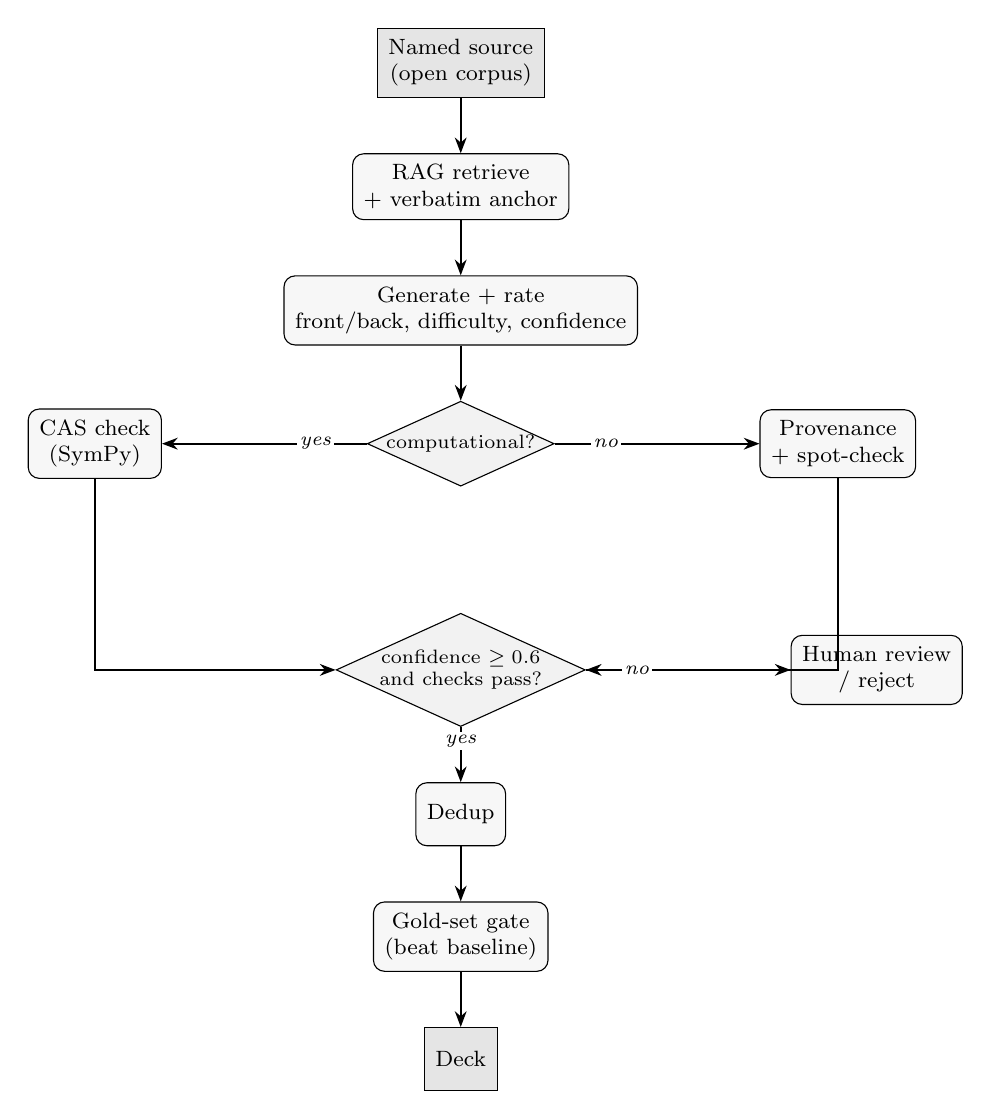
\begin{tikzpicture}[node distance=7mm and 14mm]
\node[dnode] (src) {Named source\\(open corpus)};
\node[fnode, below=of src] (rag) {RAG retrieve\\$+$ verbatim anchor};
\node[fnode, below=of rag] (gen) {Generate $+$ rate\\front/back, difficulty, confidence};
\node[dec, below=of gen] (route) {computational?};
\node[fnode, left=26mm of route] (cas) {CAS check\\(SymPy)};
\node[fnode, right=26mm of route] (prov) {Provenance\\$+$ spot-check};
\node[dec, below=16mm of route] (conf) {confidence $\geq 0.6$\\and checks pass?};
\node[fnode, right=26mm of conf] (rev) {Human review\\/ reject};
\node[fnode, below=of conf] (dedup) {Dedup};
\node[fnode, below=of dedup] (gate) {Gold-set gate\\(beat baseline)};
\node[dnode, below=of gate] (deck) {Deck};
\draw[arr] (src)--(rag); \draw[arr] (rag)--(gen); \draw[arr] (gen)--(route);
\draw[arr] (route) -- node[elbl,near start]{yes} (cas);
\draw[arr] (route) -- node[elbl,near start]{no} (prov);
\draw[arr] (cas) |- (conf);
\draw[arr] (prov) |- (conf);
\draw[arr] (conf) -- node[elbl,near start]{no} (rev);
\draw[arr] (conf) -- node[elbl,near start]{yes} (dedup);
\draw[arr] (dedup)--(gate); \draw[arr] (gate)--(deck);
\end{tikzpicture}
\caption{The generation and verification pipeline for one item. Retrieval grounding gives
provenance, a symbolic check verifies computational items while conceptual items lean on
provenance and a spot-check, low-confidence items go to human review, and a gold-set gate
governs what ships.}
\label{fig:rag}
\end{figure}

The data behind the layer is split cleanly to keep the evaluation honest. The corpus
the AI reads and cites is open, OpenStax University Physics and the Fitzpatrick texts,
chunked and embedded into about four thousand four hundred passages, each with a stable
source reference, and the keyword and vector baselines run off the same index. Real
exam forms are never fed to generation. One older form is vision-cleaned into the
problem gold ruler, two clean forms are held out as the performance bank and played in
the app's exam mode, two more are reserve held-out, and one is a sealed final mock that
also supplies the raw-to-scaled constants. Few-shot examples come from a separate clean
non-exam pool. Because nothing is both fed and graded, the beats-a-baseline-on-held-out
claim is airtight, and the dedup scan confirmed no fed example restates a real exam item.
Figure~\ref{fig:firewall} shows the split.

\begin{figure}[t]
\centering
\resizebox{\textwidth}{!}{%
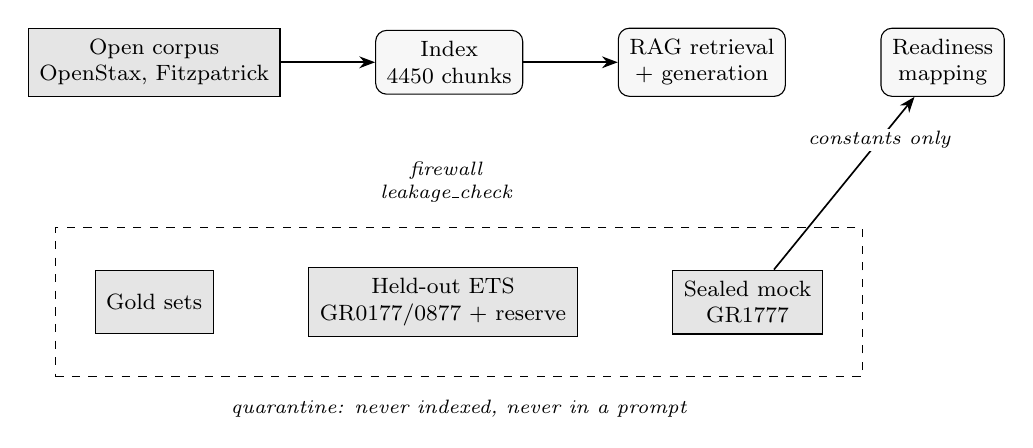
\begin{tikzpicture}[node distance=8mm and 12mm]
\node[dnode] (corpus) {Open corpus\\OpenStax, Fitzpatrick};
\node[fnode, right=of corpus] (index) {Index\\4450 chunks};
\node[fnode, right=of index] (gen) {RAG retrieval\\$+$ generation};
\node[fnode, right=of gen] (ready) {Readiness\\mapping};
\draw[arr] (corpus)--(index); \draw[arr] (index)--(gen);
\node[dnode, below=22mm of corpus] (gold) {Gold sets};
\node[dnode, right=of gold] (held) {Held-out ETS\\GR0177/0877 $+$ reserve};
\node[dnode, right=of held] (mock) {Sealed mock\\GR1777};
\node[draw, dashed, fit=(gold)(held)(mock), inner sep=5mm] (qbox) {};
\node[elbl] at ([yshift=-4mm]qbox.south) {quarantine: never indexed, never in a prompt};
\node[elbl, align=center] at ($(index)!0.5!(held)$) {firewall\\leakage\_check};
\draw[arr] (mock) -- node[elbl, near end]{constants only} (ready);
\end{tikzpicture}%
}
\caption{The leakage firewall. Only the open corpus is indexed and reachable by
generation. The gold sets, the held-out exam forms, and the sealed mock stay quarantined.
The one permitted crossing is the sealed mock's numeric score-conversion constants, used
by the Readiness mapping.}
\label{fig:firewall}
\end{figure}

\section{Evaluation}

Every model is evaluated on held-out data against a bar set in advance, and the
results are reported with their negatives. This section states the methodology, then
the results for each component. The honest boundary throughout is that this is a
single-learner project, so where a human cohort would be needed, the evaluation
validates the mechanism or the pipeline and says so. Figure~\ref{fig:eval} shows the
three held-out pipelines, one per score, that produce the numbers in this section.

\begin{figure}[t]
\centering
\resizebox{\textwidth}{!}{%
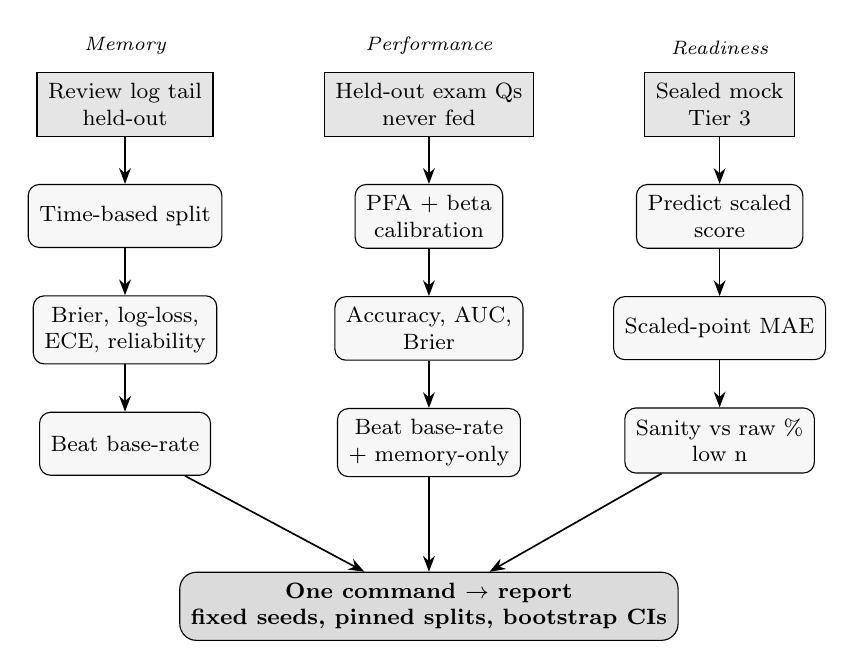
\begin{tikzpicture}[node distance=6mm and 14mm]
\node[dnode] (mrev) {Review log tail\\held-out};
\node[fnode, below=of mrev] (msplit) {Time-based split};
\node[fnode, below=of msplit] (mmet) {Brier, log-loss,\\ECE, reliability};
\node[fnode, below=of mmet] (mbase) {Beat base-rate};
\draw[arr] (mrev)--(msplit); \draw[arr] (msplit)--(mmet); \draw[arr] (mmet)--(mbase);
\node[dnode, right=of mrev] (prev) {Held-out exam Qs\\never fed};
\node[fnode, below=of prev] (ppfa) {PFA + beta\\calibration};
\node[fnode, below=of ppfa] (pmet) {Accuracy, AUC,\\Brier};
\node[fnode, below=of pmet] (pbase) {Beat base-rate\\+ memory-only};
\draw[arr] (prev)--(ppfa); \draw[arr] (ppfa)--(pmet); \draw[arr] (pmet)--(pbase);
\node[dnode, right=of prev] (rrev) {Sealed mock\\Tier 3};
\node[fnode, below=of rrev] (rmap) {Predict scaled\\score};
\node[fnode, below=of rmap] (rmet) {Scaled-point MAE};
\node[fnode, below=of rmet] (rbase) {Sanity vs raw \%\\low n};
\draw[arr] (rrev)--(rmap); \draw[arr] (rmap)--(rmet); \draw[arr] (rmet)--(rbase);
\node[term, below=12mm of pbase] (rep) {One command $\rightarrow$ report\\fixed seeds, pinned splits, bootstrap CIs};
\draw[arr] (mbase)--(rep); \draw[arr] (pbase)--(rep); \draw[arr] (rbase)--(rep);
\node[font=\scriptsize\itshape, above=1mm of mrev] {Memory};
\node[font=\scriptsize\itshape, above=1mm of prev] {Performance};
\node[font=\scriptsize\itshape, above=1mm of rrev] {Readiness};
\end{tikzpicture}%
}
\caption{The held-out evaluation, one pipeline per score. All splits are time-based,
all cutoffs and baselines are pre-registered, and one command reproduces every number
with bootstrap confidence intervals.}
\label{fig:eval}
\end{figure}

\subsection{Methodology}

Three principles govern the evaluation. Splits are time-based, never random, so no
information leaks across a card's or an item's trajectory \citep{kapoor2023}. Cutoffs
and baselines are pre-registered, frozen and dated before results are seen. Runs are
reproducible from one command with fixed seeds, and every metric is reported with a
bootstrap confidence interval. The primary calibration metric is the Brier score,
which is binning-free, supported by log-loss, the expected calibration error, and a
reliability diagram, which can disagree at small samples and so are reported together.

The scoring process is built to keep the numbers honest. Items from every system, the
AI and each baseline, are shuffled together and scored blind to their source, so a
rater cannot favor the AI. Two raters score each batch, a human and an AI judge, the
human adjudicates disagreements, and inter-rater agreement is reported alongside the
scores. Every run is driven by one command with fixed seeds and pinned splits, and each
headline number carries a bootstrap confidence interval, so the whole evaluation
reproduces from the same inputs.

\subsection{Memory calibration}

Memory is calibrated on a held-out tail of a large public review-log dataset
\citep{ankirevlogs2024}, where the model predicts retrievability and the log records
the actual pass or fail. On the held-out split, Memory reaches a Brier score of
$0.234$, a log-loss of $0.743$, and an expected calibration error of $0.159$, and it
beats the base-rate baseline on the primary Brier score. The reconstruction is pinned
to the exact memory-model version the engine ships, so the calibration reflects the
deployed model.

\subsection{Performance}

With one learner there is not yet a bank of the learner's own attempts on novel items
large enough to fit and validate a logistic model honestly. The Performance pipeline
is therefore validated on a seeded, documented synthetic dataset whose outcomes are
drawn from a known logistic process, which validates the fitting, calibration, and
held-out machinery rather than a human effect. On the held-out synthetic split, the
calibrated model reaches a Brier score of $0.175$ and an accuracy of $0.775$, against
$0.268$ and $0.563$ for the base-rate baseline, and the pre-registered
beat-the-baseline rule passes. The report states plainly that this validates the
pipeline at a sample size of one, and that real coefficients need a real cohort.

\subsection{Readiness}

Readiness maps expected performance to the 200 to 990 scale with an 80\% range and is
coverage-gated at 70\%. With one or two practice forms available, the check of
predicted against actual scaled score is a sanity check, reported as such rather than
as a full validation. The mechanism of interest, the coverage gate and the abstain
behavior, is the part that is verifiable now, and it behaves as specified: below the
coverage line, Readiness abstains and names the uncovered exam.

\subsection{The AI layer}

The AI gate was scored on a batch against 157 verified gold items, with generation
from a pinned model and two blind raters. Table~\ref{tab:eval} includes the headline
numbers. Under the human adjudicator, generated cards reach a useful-yield of $0.84$,
clearing the $0.80$ bar, with a fact precision of $0.90$, one step under the $0.95$
floor because five cards carried a fact slip. The non-refused problems are excellent
by the human rater (key correctness $1.00$, useful-yield $0.92$, distractor quality
$0.96$), but a 31\% problem refusal rate, mostly malformed or declined generations
plus a smaller share of answer-leak safeguards, drags the batch numbers under the
bars. The AI beats keyword and vector retrieval by $0.74$ on cards and $0.67$ on
problems, and beats naive-distractor generation by $0.42$, all with confidence
intervals excluding zero, which is the spec's core requirement and validates the
misconception-first design.

Two findings deserve emphasis. First, the two absolute quality cutoffs that remain
short (card fact precision and the problem batch yield) are generation issues, cutting
the malformed-problem rate and tightening fact precision, not gold-set or methodology
problems. Second, the human and AI judges barely agreed, with a Cohen's kappa of
about $-0.03$ on usefulness. The AI judge systematically under-rated usefulness, so an
AI-only gate would have been unreliable here. That near-zero agreement is itself a
result, and it is the clearest argument for the two-rater rule.

Two process details support these numbers. Between an initial pass and the scored run,
the generator gained key self-consistency, an independent re-solve that regenerates a
problem when its own solution disagrees with the key, and a tuned grounding floor, which
together roughly halved refusals and lifted problem key-correctness under the AI judge.
The firewall held throughout: no exam form was fed, and a reject-memorized check kept
all eighty-six candidate items, none a near-copy of a fed example, with the
seen-versus-held split recorded in the run manifest.

\begin{table}[t]
\centering
\small
\begin{tabular}{@{}p{2.6cm}p{3.5cm}p{2.6cm}p{4.4cm}@{}}
\toprule
\textbf{Model} & \textbf{Metric (held-out)} & \textbf{Result} & \textbf{Baseline and note} \\
\midrule
Memory & Brier / log-loss / ECE & 0.234 / 0.743 / 0.159 & Beats base-rate on Brier; real review logs \\
Performance & Brier / accuracy & 0.175 / 0.775 & 0.268 / 0.563 base-rate; synthetic, n=1 pipeline check \\
Readiness & Scaled 200--990, 80\% range & Coverage-gated & Sanity check only, low n \\
AI cards & Useful-yield / fact precision & 0.84 / 0.90 & +0.74 vs retrieval; fact precision one step under bar \\
AI problems & Key / useful / distractor & 1.00 / 0.92 / 0.96 & Non-refused; +0.67 vs retrieval, +0.42 vs naive; 31\% batch refusal \\
\bottomrule
\end{tabular}
\caption{Evaluation results. All comparisons are held-out; confidence intervals for
the AI advantages exclude zero.}
\label{tab:eval}
\end{table}

\subsection{The interleaving ablation}

The study feature is ablation-tested in a controlled simulation. With one learner
there is no cohort, so the ablation validates the shipped selection mechanism under
the memory model as ground truth, and does not establish a human interleaving effect.
The pre-stated primary metric is blueprint-weighted expected recall at the exam
horizon, which is the app's actual objective and is coverage-aware. Three arms study
for equal time: the full interleaved selector, a blocked (massed) arm, and stock
scheduling in soonest-due order. Table~\ref{tab:ablation} gives the grid across study
budget and exam distance.

Two results stand out, and one non-result. The full selector beats massed practice in
every configuration, by $0.008$ to $0.075$, with every confidence interval excluding
zero. This is the core learning-science claim, that spaced topic-mixed practice beats
massed practice, and it holds robustly. Against stock scheduling, the full selector
wins at every realistic study budget, 20 and 30 reviews per day, including the
headline configuration where it leads by $0.015$. It loses only at the tightest
budget, 10 reviews per day, and the reason is mechanical and expected: the
desirable-difficulty band reviews cards below their soonest-due point, spending
near-term recall to buy long-term stability, a trade that does not pay back when the
budget is too small to review much at all. The non-result is that the anti-blocking
reshuffle registers as exactly zero under this memory model, because same-day review
order does not change the model's updates. Its justification is cognitive, about
discrimination and contextual interference, which this simulation cannot capture, so
it is neither credited nor refuted here.

The comparison is controlled rather than casual. Every arm studies for exactly the same
number of reviews, common random numbers pair the recall outcomes across arms so the
arms differ only in their ordering, and the intervals are bootstrapped over forty seeds.
The honest read of the blocked contrast is that it tests spaced-mixed versus massed
practice, because the full arm also prioritizes within a topic by weakness, so the win
over blocked is the broad interleaving effect rather than a single-variable swap. At the
headline budget the full arm's per-area recall is uniformly high across all nine
blueprint areas, which is what a coverage-aware objective should produce.

\begin{table}[t]
\centering
\small
\begin{tabular}{@{}cccc@{}}
\toprule
\textbf{Budget (reviews/day)} & \textbf{Exam gap (days)} & \textbf{full $-$ blocked} & \textbf{full $-$ stock} \\
\midrule
10 & 0  & $+0.011$ & $-0.037$ \\
10 & 90 & $+0.008$ & $-0.023$ \\
20 & 0  & $+0.068$ & $+0.005$ \\
20 & 90 & $+0.062$ & $+0.005$ \\
30 & 0  & $+0.075$ & $+0.015$ \\
30 & 90 & $+0.074$ & $+0.014$ \\
\bottomrule
\end{tabular}
\caption{Ablation grid. Positive means the full selector is better. Every confidence
interval excludes zero. The full selector beats massed practice everywhere and beats
stock scheduling at realistic budgets, losing only at the tightest budget.}
\label{tab:ablation}
\end{table}

\subsection{Two-way sync}

The two-device requirement is met by reusing the engine's own sync unmodified against
a self-hosted server. Reviews and problem attempts union by identifier, so two devices
reviewing different cards offline both land with nothing lost or double-counted, and
for the same card on both devices the newer modification time wins the scheduling
state. A round-trip test covers different cards offline, the same card on both, the
attempt-log union, and offline-then-sync, and an on-device path uploads a review from
the phone that the desktop then downloads. The conflict rule is the engine's own, made
explicit rather than reinvented: review history and the attempt log are append-only and
union by identifier, so nothing is lost or double-counted, while for the same card
edited on both devices the newer modification time wins the scheduling state, with a
deterministic device tie-break on equal times. Offline safety rides the engine's
transactional store, so a session works fully offline and syncs opportunistically, and
a kill-mid-review stress test leaves the collection uncorrupted.

\section{Discussion}

The through-line of pgrep is honesty by construction. The coverage gate and the
abstain rules mean the system cannot present a readiness number over an unpracticed
part of the exam, so a confident-looking but empty score is not a risk to be avoided
by discipline, it is impossible by design. Every score ships a range and states its
evidence, which is the practical form of preferring calibration to confidence.

The ablation illustrates the same posture applied to the authors' own feature. The
selector's clean, robust win is over massed practice, the mechanism the literature
actually supports. Against stock scheduling the win is real at realistic budgets but
not universal, and the one loss is explained rather than hidden. A study tool that
spends near-term recall to buy durable stability should be expected to lose when the
learner can barely review, and it does. Reporting that makes the wins credible.

The AI evaluation produced a methodological result the project did not set out to
find. The human and AI judges agreed at close to chance, and the AI judge
under-rated usefulness. Had the gate relied on the AI judge alone, it would have
rejected good material. The two-rater rule, adopted in advance for integrity, turned
out to be load-bearing. This is a small but concrete case for keeping a human in the
loop on generative-quality gates.

Finally, AI is an upgrade and not a dependency. The three scores are pure arithmetic
over the memory model and the attempt log, the tutor has a stored-decomposition
fallback, and an AI-off session loads none of the generative code. The system that
ships and scores is the system without AI, and AI improves it where it is available
and trustworthy.

The data-model decision is a quiet instance of the same discipline. Storing the attempt
log as notes rather than a custom table cost a little analytic convenience, but it
bought two-way sync for free and kept the most heavily weighted requirement, correct
multi-device sync, out of reach of a bug in hand-written sync code. The pre-engineered
but unbuilt cache means the convenience can be recovered later without touching sync.
Choosing the boring option that protects the load-bearing requirement is, in miniature,
the whole posture of the project.

pgrep also sits in a specific relationship to the tool it reuses. A stock
spaced-repetition application answers one question well, will you recall this card, and
answers it with a strong memory model. pgrep keeps that answer intact and adds the two
questions an exam candidate actually asks, can I apply it and what will I score, without
disturbing the memory model underneath. The contribution is not a better scheduler, it
is the readiness layer and the honesty machinery built on a scheduler that was already
good.

Several threads are ready to pick up. The readiness-aware weighting of the selector is
designed but not shipped. The Performance model awaits a real attempt history to fit
true coefficients, at which point the same held-out harness that validated the pipeline
validates the model itself. The two short AI cutoffs are a generation problem, cutting
the malformed-problem rate and tightening fact precision, not a change to the bar. And
the calibration measured offline here can be surfaced live as the attempt log grows.

\section{Limitations}

The central limitation is sample size. pgrep is validated by one learner, so several
results are mechanism-level rather than population-level. The Performance model is
validated on synthetic data, which exercises the pipeline but does not establish the
learner's true coefficients. The interleaving ablation is a simulation under the
memory model as ground truth, not a human trial, and its anti-blocking arm is invisible
to that model by construction. The simulation also collapses ratings to pass or lapse
and assumes the selector's predicted recall equals the ground-truth recall, which
isolates ordering from calibration error but idealizes it. The Readiness check against a real form is a low-sample
sanity check. On the AI layer, two absolute quality cutoffs remain just short, card
fact precision and the refusal-limited problem batch yield, and closing them is
generation work still to do. The literature cited here was assembled from the
project's working notes, and a citation-verification pass for exact figures and
identifiers is pending before any external use. None of these undercut the reported
numbers, but they bound what those numbers mean.

\section{Conclusion}

pgrep is a Physics GRE preparation system that treats readiness as a measurement
problem. It reorders study by exam value inside the engine, it reports three separate
and calibrated scores that never confuse recall with transfer, and it generates
practice items that cite a named source or refuse, all validated on held-out data and
all still working with AI switched off. The evidence supports specific claims and no
more: Memory calibrates and beats its baseline on real review logs, the selector beats
massed practice everywhere and stock scheduling at realistic budgets, and the AI layer
beats every baseline while two absolute quality bars remain in reach. Stated that
precisely, the system does what it claims, and it says so honestly where it does not.

\section*{Data Availability}

The bundled corpus is openly licensed (OpenStax University Physics and the Fitzpatrick
texts). Official exam forms used for held-out validation and as a grading ruler are
copyright and are never bundled, shipped, indexed, or fed to generation; only numeric
score-conversion constants are used, and they stay in a private workspace. The private
evaluation workspace (corpus index, gold items, held-out forms, and harness) is not
distributed. Aggregate results and the evaluation harness are reproducible from a
single command with fixed seeds.

\section*{Ethics and AI-Use Disclosure}

pgrep uses large language models in two places, and this report discloses both. In
the product, AI generates study items and tutoring, governed by provenance,
gold-set gating, and a leakage firewall, and disabled by default. In the preparation
of this report, an AI assistant helped organize source material and draft prose from
the project's own documentation and recorded results; all numbers trace to the
project's evaluation artifacts, and the author is responsible for the content. The
system inherits and preserves the reused engine's AGPL license and its attribution.

\bibliographystyle{apacite}
\bibliography{references}

\end{document}
